\chapter{IoT Design}

In software architecture, the publish/subscribe pattern is a messaging pattern where senders of messages (publishers), do not program the messages to be sent directly to specific receivers (subscribers), but instead categorize published messages into topics without knowledge of which subscribers, if any, there may be. Subscribers express interest in one or more topics, and only receive messages that are of interest, without knowledge of which publishers, if any, there are. This pattern decouples senders and receivers, allowing for greater scalability and a more dynamic communication environment.\vspace{5mm} \\
Eclipse Mosquitto is an open-source message broker software that implements the \gls{mqtt} protocol, a standard for publish/subscribe messaging for the \gls{iot}. Mosquitto provides a lightweight way for IoT devices to communicate with each other, allowing them to publish and subscribe to messages on topics. With Mosquitto, devices can publish information, such as sensor readings or status updates, to the message broker and receive updates from other devices. Mosquitto helps to facilitate efficient and effective communication between \gls{iot} devices in a scalable manner.\vspace{5mm} \\
Table \ref{iot-table} identifies functions excuted by microcontrollers and the \gls{iot} messaging attributes.\vspace{5mm} \\

\begin{table}[!ht]
    \begin{center}
    \begin{tabular}{|l|l|l|l|}
    \hline
        \textbf{Micro Function} & \textbf{Pub/Sub} & \textbf{Topic} & \textbf{Message} \\ \hline
        RFID Reader & Pub & sensors/rfid & RFID \\ \hline
        Turnout Contacts & Pub & sensors/toc & Turnout Position\\ \hline
        Turnout Panel Push Button & Pub & sensors/pb & TP Button \\ \hline
        Heartbeat & Pub & micros & Micro Info\\ \hline
        Turnout & Sub & acts/to/cntrlr id &  Turnout Cmd\\ \hline
        Turnout Panel Light & Sub & acts/tpl/cntrlr id & TP Light Cmd\\ \hline
        Micro Info & Pub & micros & Micro Info\\ \hline
    \end{tabular}
    \caption{\label{iot-table}IoT Micro Function Table}
    \end{center}
\end{table}

Figure \ref{fig:iotdesign} depicts the flow of \gls{mqtt} messages through the \gls{mqtt} broker from and to microservices components.

\begin{figure}[H]
	\centering
		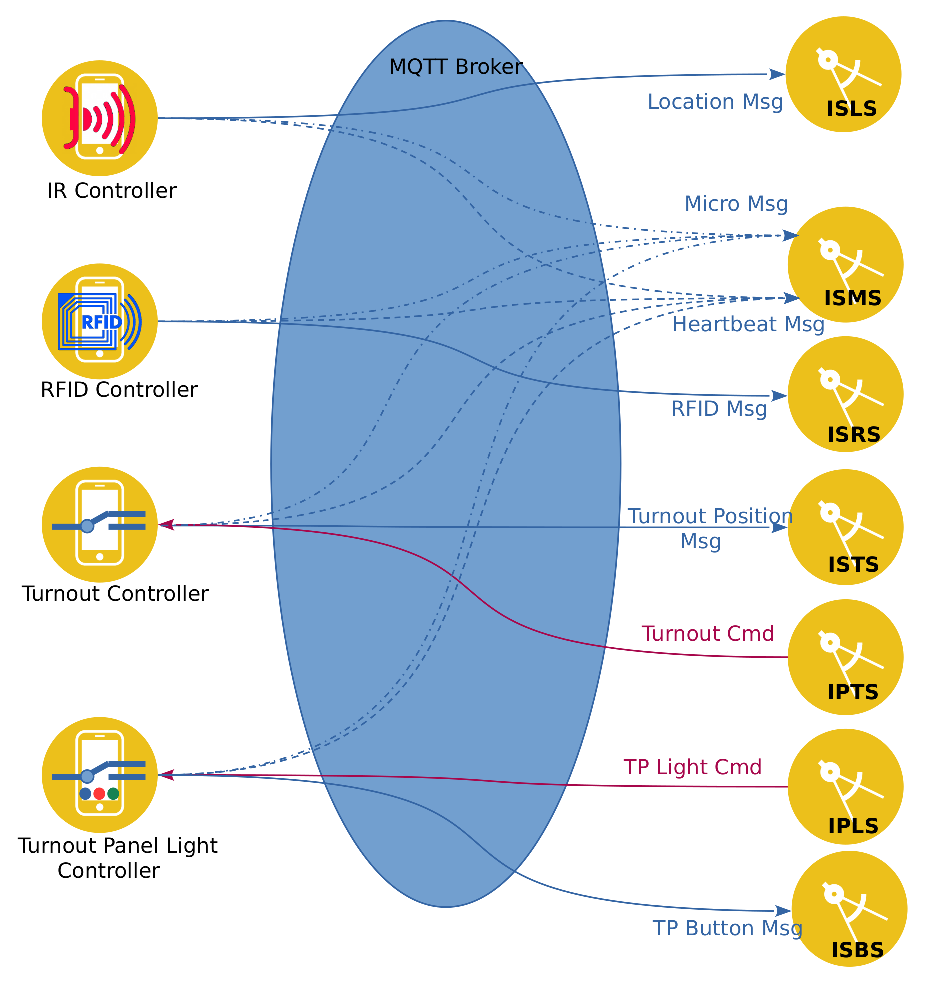
\includegraphics[scale=0.7]{mqtt-v7.eps}
	\caption{IoT Design}
	\label{fig:iotdesign}
\end{figure}

\section{Message Definitions}
\begin{itemize}
\item \textbf {\gls{rfid}} message format: \{“et”:“epoch time",”mcntrlr”:”sensor id“,”rfid”:”rfid tag value“\}
\begin{itemize}
\item example \{"et":"1590463450",”mcntrlr”:"rfidRdr01","reader":"1","rfid":"1C0044CF23"\}
\end{itemize}
\item \textbf {Turnout Position} message format: \{“et”:”epoch time“,”mcntrlr”:”turnout controller id“, \\”to”:”turnout number“,”state”:”THROWN|CLOSED|ERROR“\}
\begin{itemize}
\item example \{"et":"1588827073",”mcntrlr”:"TrnCtlr01","to":"1","state":"THROWN"\}
\end{itemize}
\item \textbf {Turnout Panel Button} message format: \{“et”:”epoch time“,”mcntrlr”:”tp controller id“, \\”pb”:”push button number“\} 
\item \textbf {Turnout Command} message format: \{”mcntrlr”:”turnout controller id“,”to”:”turnout number“, \\”cmd”:”THROW|CLOSE|STATUS“\}
\begin{itemize}
\item example \{”mcntrlr”:"TrnCtlr01","to":"1","cmd":"CLOSE"\}
\end{itemize}
\item \textbf {Turnout Panel Light Command} message format: \{”mcntrlr”:”turnout panel controller id“, \\”tpl”:”light number“,”color”:”RED|GREEN|BLUE“,”type”:”BUTTON”\}
\item \textbf {Micro Info} message format: \{“et”:”epoch time“,”mcntrlr”:microcontroller id“, \\"msgType":"initial|heartbeat","ip":"Address of Micro"\}
\begin{itemize}
\item 'heartbeat' example: \{"et":"1590462747",”mcntrlr”:"RfidRdr00","msgType":"heartbeat"\} 
\item 'initial' example: \{"et":"1590462747",”mcntrlr”:"RfidRdr00","msgType":"initial","ip":"192.168.0.19"\}
\end{itemize}
\end{itemize}
